\documentclass[12pt,twoside]{report}
\usepackage[utf8]{inputenc}
\usepackage{polski}
\usepackage{mathtools}
\DeclarePairedDelimiter{\abs}{\lvert}{\rvert}
\usepackage{graphicx}
\usepackage[section]{placeins}
\usepackage{caption}
\usepackage{gensymb}
\usepackage{subcaption}
\usepackage[a4paper,width=150mm,top=25mm,bottom=25mm,bindingoffset=6mm]{geometry}
\usepackage{fancyhdr}
\usepackage{listings}
\linespread{1.3}
\pagestyle{fancy}
\fancyhead{}
\fancyhead[RO,LE]{System przetwarzania danych wektorowych oparty na układzie FPGA}
\fancyfoot{}
\fancyfoot[LE,RO]{\thepage}
\fancyfoot[LO,CE]{Rozdział \thechapter}
\fancyfoot[CO,RE]{Dyczek, Moczurad}
\renewcommand{\headrulewidth}{0.4pt}
\renewcommand{\footrulewidth}{0.4pt}
\title{Thesis Title}
\author{Author Name}
\date{Day Month Year}	

\begin{document}
	\begin{titlepage}
    \begin{center}
		\fontsize{17pt}{20pt}\selectfont
        \textbf{Akademia Górniczo-Hutnicza\\im. Stanisława Staszica w Krakowie}
        \rule{\textwidth}{1.5pt}\par
        \vspace{0.5cm}
        Wydział Informatyki, Elektroniki i Telekomunikacji
        
        \vspace{1.5cm}

        \includegraphics[scale=0.75]{images/agh}
 		
 		\vspace{1.5cm}
 		
 		Dokumentacja użytkownika
 		
 		\vspace{0.5cm}
	 	\textbf{Sprzętowo-programowy system\\przetwarzania danych wektorowych,\\oparty na ukladzie FPGA}
		
		Piotr Moczurad
		Tomasz Dyczek
		\vspace{1.5cm}\\
		\textbf{Opiekun}\\
		dr inż. Jacek Długopolski
		\rule{\textwidth}{1.5pt}\par
		Kraków 2015
		
        
    \end{center}
\end{titlepage}
	\tableofcontents	
	
	\chapter{Metodyka}
    \section{Struktura projektu}

Struktura projektu, a wraz z nią struktura repozytorium, odzwierciedla wyraźny podział na część software'ową (kompilator naszego języka programowania) oraz hardware'ową (koprocesor zaimplementowany na układzie FPGA). Dodatkowo, dokumentacja do projektu jest również trzymana w repozytorium, co umożliwia łatwiejszą współpracę nad jej tworzeniem i pozwala na zarządzanie jej wersjami.

Część hardware'owa, związana z FPGA, ma niemalże płaską strukturę: mamy jeden moduł główny i kilka pomniejszych komponentów, które są do niego dołączone (jako osobne części układu zaimplementowane są jego wyróżnione składowe, takie jak stos, pamięć ram czy moduł UART). Każdy z komponentów umieszczony jest w oddzielnym pliku.

Część software'owa jest w pełni autonomicznym projektem języka Haskell, budowanym systemem budowania Cabal. Narzuca to pewną strukturę plików i katalogów (w Haskellu tworzone są hierarchiczne moduły poprzez umieszczanie plików w odpowiednich ścieżkach folderów). Projekt podzielony jest na części związane z etapami kompilacji programów w naszym języku, w szczególności na dwa główne moduły: \texttt{Parser} i \texttt{CodeGen}, które z kolei podzielone są na bardziej szczegółowe submoduły. Dokładna struktura plików i katalogów została przedstawiona na rysunku \ref{fig:file_structure}.

\begin{figure}
  \begin{center}
    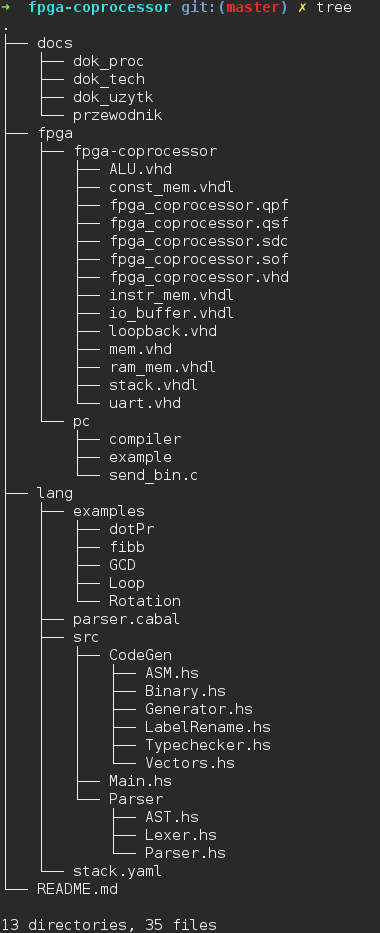
\includegraphics[scale=0.5]{images/file_structure.png}
    \caption{Struktura plików w projekcie jako wynik polecenia \texttt{tree} w systemie Linux.}
    \label{fig:file_structure}
  \end{center}
\end{figure}

\section{Porady dotyczące budowania}

Zwykły użytkownik systemu nie musi zajmować się jego budowaniem, jednak programista, pragnący rozwijać system, musi zapoznać się ze specyfiką budowania projektów języka Haskell w systemie Cabal oraz języka VHDL w środowisku Quartus.

\subsection{Haskell}
Cały projekt haskellowy mieści się w katalogu \texttt{lang}. Pierwszą rzeczą, na którą należy zwrócić uwagę jest plik \texttt{parser.cabal}. Jest to plik opisujący projekt Cabala, który służy nam m.in. do określania zależności projektu wraz z ich wersjami, dostarczania informacji o projekcie, ustawiania globalnych opcji kompilacji dla całego projektu, czy włączania rozszerzeń języka Haskell na poziomie projektu. W pliku tym możemy zdecydować, czy projekt ma być budowany jako biblioteka (\textit{library}) czy wykonywalny program (\textit{executable}). Możemy również, jak w przypadku naszego projektu, zbudować projekt na obydwa sposoby. Dla obydwu rodzajów budowania podajemy katalogi, w których kompilator ma szukać plików źródłowych (\texttt{hs-source-dirs}), opcje kompilatora (\texttt{Ghc-Options}) i zależności (\texttt{build-depends}).

Zależności są polem, na które warto zwrócić szczególną uwagę. W przeciwieństwie do systemów budowania języka Java, takich jak Maven, Cabal nie ściąga archiwów \texttt{.jar} z bibliotekami. Ściąga jedynie źródła, które potem kompiluje. Tworzy to pewne problemy z wersjami bibliotek (wyobraźmy sobie sytuację, w której biblioteka $A$ wymaga biblioteki $B$ w wersji 0.1 oraz biblioteki $C$ w wersji 0.2, a z kolei biblioteka $B$ wymaga biblioteki $C$ w wersji 0.3 --- problemy z wersjami bibliotek są powszechne przy stosowaniu Cabala), które możemy próbować obchodzić przez wymuszanie konkretnych wersji bibliotek lub ich przedziałów. W naszym projekcie jednak wybór padł na używanie wszystkich bibliotek w ich najnowszych wersjach, więc żadne wersje nie są sztucznie wymuszane. Jest to możliwe również dzięki zastosowaniu technologii \textit{sandboxów}. Zamiast instalować wszystkie biblioteki globalnie do systemu (co potencjalnie rodzi konflikty, jeśli mamy więcej niż jeden projekt), instalujemy je do osobnego środowiska umieszczonego w osobnym folderze, które możemy łatwo usunąć i odtworzyć w razie problemów.

Po zainstalowaniu projektu poleceniem \texttt{cabal install} utworzy się folder \texttt{dist}, w którym można znaleźć pliki wykonywalne i biblioteki utworzone podczas budowania. Popularną praktyką wśród programistów Haskella jest usuwanie katalogu \texttt{dist} w razie problemów z budowaniem i \texttt{.cabal-sandbox} w razie problemów z wersjami pakietów.

\subsection{FPGA}

Projekt FPGA jest utworzony w środowisku Quartus II firmy Altera, które automatyzuje budowanie projektu przez dostarczenie zintegrowanego środowiska do projektowania i syntezy układów. Kompilacja odbywa się za pomocą graficznego interfejsu i nie wymaga szczegółowego opisywania. W razie problemów z kompilacją Altera dostarcza obszerną dokumentację do środowiska Quartus. Ważnym plikiem jest \texttt{fpga\_coprocessor.qsf}, który zawiera przypisania pinów (\textit{pin assignments}) dla projektu. W przypadku budowania projektu dla innej płytki, niż Altera De0-Nano, należy zmienić plik tak, by nazwy pinów odpowiadały tym, które faktycznie są dostępne na płytce. Jest to o tyle istotne, że w przypadku rozszerzania układu może zajść konieczność użycia większej płytki (z większą ilością elementów logicznych i szybszym wejściem-wyjściem).

\subsection{Komunikacja}

Aby skompilować prosty program do obsługi komunikacji z koprocesorem, który można znaleźć w katalogu \texttt{fpga/pc} wystarczy zwyczajny kompilator języka C. Przy tworzeniu projektu wykorzystano kompilator GCC w wersji 5.1, choć każdy kompilator obsługujący standard C99 wystarczy do skompilowania programu. Przykładowe polecenie to: \texttt{gcc -o sender sender.c}. Dodatkowo, komunikacja odbywa się przez port szeregowy, więc trzeba zadbać, by urządzenie w systemie, jako które widoczny jest nasz port, było faktycznie rozpoznawane przez system jako port szeregowy. Służy temu polecenie \texttt{setserial}, dostępne w systemach linuksowych po zainstalowaniu pakietu o tej samej nazwie. Przykładowo, używając systemu Fedora 22 musimy wydać polecenie: \texttt{sudo dnf install setserial \&\& sudo setserial -g /dev/ttyUSB0}. W powyższych instrukcjach bazujemy na założeniu, że do komunikacji używana jest przejściówka USB-UART. Jeśli do rozwoju systemu zostanie użyty inny sposób podłączenia (np. bezpośrednio do pinów GPIO na urządzeniach typu Arduino bądź Raspberry Pi), nazwa urządzenia może ulec zmianie.


    \chapter{Przebieg prac}
    Jak wspomniano w rozdziale pierwszym, przebieg prac i etapy realizacji korespondują z kolejnymi spotkaniami projektowymi.
\begin{table}[!ht]
\begin{tabular}{|l|l|} \hline
Etap & Opis\\ \hline
1 & Projektowanie składni i systemu typów języka oraz architektury procesora. \\
  & Analiza istniejących procesorów opartych na FPGA\\  \hline
2 & Implementacja języka programowania i kompilatora \\
  & Zmiany w koncepcji dotyczącej procesora\\ \hline
3 & Implementacja modułu komunikacyjnego oraz procesora\\
  & Dalszy rozwój kompilatora \\ \hline
4 & Drobne poprawki w całym projekcie\\
  & Opracowanie przykładów działania, dokumentacja\\
\hline
\end{tabular}
\end{table}

\section{Etap pierwszy}
Pierwszy etap rozpoczął się po marcowym spotkaniu z prowadzącym. Wymagał on zagłębienia się w tematykę teorii kompilacji i budowy procesorów, w szczególności istniejących gotowych rozwiązań dla FPGA. Naszym celem było odpowiednie zaprojektowanie języka oraz dobór odpowiednich narzędzi do jego parsingu, transformacji i translacji do asemblera. Część sprzętowa wymagała wyboru i zaopatrzenia się w odpowiedni zestaw startowy oraz sprzęt do komunikacji komputer-FPGA. Należało też dokonać wyboru pomiędzy językami opisu sprzętu - Verilogiem a VHDLem. Istotną kwestią był taki sposób zaplanowania przedsięwzięcia by później - podczas implementacji procesora - nie okazało się, że zakupione zestawy startowe posiadają zbyt małą ilość bramek logicznych do realizacji założeń początkowych.
\subsection{Realizacja etapu}
Podjęliśmy decyzję o implementacji kompilatora w języku Haskell. Z wcześniejszych doświadczeń wiedzieliśmy, że język ten jest wyjątkowo dobrze przystosowany do trawersacji po strukturach i innych zadań powiązanych z kompilatorami. Do parsowania wybraliśmy bibliotekę parsec, do binaryzacji pakiet binary. Zdecydowaliśmy też o semantyce języka - stwiedziliśmy, że należy dać użytkownikowi możliwość użycia 2 typów zmiennych - liczb całkowitych i wektorów liczb. Wybraliśmy potrzebne elementy języka - pętle i instrukcje warunkowe. Zdecydowaliśmy o składni oraz formatowaniu i znakach białych. W kwestiach sprzętowych zdecydowaliśmy, że procesor zrealizujemy na zestawach startowych Terasic DE0-Nano które będą odbierały program kompilowany na platformach komputerowych Raspberry PI. Do komunikacji pomiędzy Raspberry PI a FPGA wybraliśmy układ UART. Zapoznaliśmy się z pracami na temat implementacji procesorów na FPGA oraz z ich konkretnymi przykładami.  
\section{Etap drugi}
Drugi etap rozpoczął się po spotkaniu w czerwcu na którym przedstawiliśmy skonkretyzowaną wizje projektu. Na spotkaniu zaproponowana została koncepcja procesora stosowego oraz podziału wektora o zmiennej długości na mniejsze. W ramach drugiego etapu planowaliśmy rozpocząć tworzenie kompilatora - rozpoczynając od parsera oraz prostego typecheckera. Mieliśmy również nadzieje rozpocząć prace nad pierwszą wersją tłumaczenia AST do asemblera. Planowaliśmy realizacje prototypowej komunikacji z użyciem UART.
\subsection{Realizacja etapu}
Udało nam się napisać parsera języka oraz zaprojektować dla niego odpowiednie AST. Zaimplementowaliśmy prosty moduł type-checkujący. Zaprojektowaliśmy pierwotną wersje asemblera z wykorzystaniem arbitralnej ilości rejestrów. Napisaliśmy moduł tłumaczący drzewo AST do ASM oraz zaimplementowaliśmy obsługę instrukcji warunkowych w ASM. Podjeliśmy też bardzo istotną decyzję dotyczącą kwestii sprzętowych - uznaliśmy, że kompilowanie programów na platformie Raspberry PI nie jest w realizacji projektu potrzebne. Zamiast tego zakupiliśmy konwertery USB-UART umożliwiające komunikacje wysyłanie i odbieranie danych z komputera poprzez wirtualny port COM. Dzięki temu udało się nam z projektu wyłączyć dodatkowy element jakim była obsługa Raspberry PI. Dokonaliśmy zmiany koncepcyjnej w architekturze assemblera i procesora - zdecydowaliśmy, że zamiast zwykłych rejestrów zaimplementujemy procesor stosowy co w znaczącym stopniu uprości kompilacje programów oraz zmniejszy ilość potrzebnych mnemoników. Zaimplementowaliśmy obsługę UART po stronie FPGA oraz PC. Przesłaliśmy pierwsze dane przez interfejs USB-UART. Udało nam się już w drugim etapie podjęcie prac nad procesorem w VHDL. Rozpoczęliśmy implementacje pierwszych stanów w maszynie stanowej FPGA oraz potrzebnych struktur - tablic pamięci oraz stosów. Rozpoczęliśmy analizę obsługi wektorów - podjęliśmy decyzję o przetwarzaniu ich w postaci 8 elementowych kawałków. Stworzyliśmy pierwszy - prototypowy - moduł dokonujący tłumaczenia asemblerowych mnemoników do postaci binarnego pliku - programu.
\section{Etap trzeci}
Trzeci etap rozpoczął się po październikowym spotkaniu dotyczącym działania procesora. Planowaliśmy w nim rozstrzygnąć pytania dotyczące procesora - kształ i działanie koprocesora arytmetycznego oraz działanie rejestrów wektorowych na które kopiowalibyśmy wektory przed rozpoczęciem obliczeń. Najważniejszym zadaniem była implementacja procesora dla urządzenia startowego. Chcieliśmy zbudować go inkrementalnie - tzn. dodawać kolejne stany maszyny tak by obsługiwały coraz bardziej złożone mnemoniki asemblera.
\subsection{Realizacja etapu}
Podjęliśmy decyzję o całkowitym zmodyfikowaniu modułu binaryzacji instrukcji asemblera. Jak nam poradzono przerobiliśmy instrukcje tak aby miały stałą długość natomiast stałe wykorzystane w programie doklejane były na koniec pliku binarnego. Zaimplementowaliśmy również nową - lepszą i bardziej odporną na błędy -  obsługę UART po stronie FPGA. Zaczęliśmy łączyć kolejne moduły VHDL w całość - pamięć na stałe liczbowe, pamięć intrukcji, stos wektorów. Zaimplementowalimy 2 stosy-rejestry na wektory. Następnie tak jak założyliśmy - inkrementalnie dodawaliśmy obsługę kolejnych komend - kopiowania wartości zmiennych do i z pamięci, kopiowanie danych ze stosu, itd. Zaimplementowaliśmy koprocesor arytmetyczny wykonujący wszystkie możliwe operacje na raz dla wektorów. Rozszerzyliśmy procesor o obsługę bardziej złożonych operacji - skoków JMP i mnemoników warunkowych (IF, IFZ). Dodaliśmy stany umożliwiające odsyłanie danych wyjściowych. Zmodyfikowaliśmy koncepcje dotyczące pętli LOOP. Od tej pory jest ona jedynym wyrażeniem nie zwracającym żadnej wartości. Zaimplementowaliśmy w języku C program obsługujący wysyłanie i odbieranie wyników programów z komputera wraz z obsługą błędów. Udało się nam przesłać przykładowe programy które zwracały poprawne wartości. Zaimplementowaliśmy przykładowe programy sprawdzające ogólne działanie programu, wykonujące dużą ilość iteracji. Zaimplementowaliśmy program liczący kolejne liczby fibonacciego w celu przedstawienia na kolejnym spotkaniu projektowym.
\section{Etap czwarty}
Czwarte spotkanie projektowe dotyczyło konkretnych przykładów obliczeń jakie mielibyśmy zaprezentować na procesorze. W danym etapie planowaliśmy rozszerzenie ilości obługiwanych operacji o 3 kolejne. Chcieliśmy również poprawić pewne błędy języka i ułatwić proces kompilacji oraz wysyłania programu. 
\subsection{Realizacja etapu}
Dodaliśmy do języka 3 nowe elementy drzewa syntaktycznego - operację rot90, scalarProd oraz modulo. Rozszerzyliśmy również asembler o wektorowe wsparcie dla tych operacji. Przy dobieraniu funkcji kierowaliśmy się tym jakie rzeczywiste operacje mógłby chcież wykonać użytkownik. I tak - rot90 - rotacja została dodana w celu pokazania łatwości rozszerzalności procesora o kolejne najróżniejsze komendy. Operacja scalarProd jest iloczynem skalarnym i dodanie jej umotywowaliśmy faktem, że w rzeczywistych obliczenia jest bardzo często używana. Również operacje modulo dodaliśmy mając na uwadze jak istotnym jest ona elementem obliczeń. Na końcu zaimplementowaliśmy w rozwijanym przez nas języku przykładowe programy pokazujące poprawność działania ale i przydatnośc wymienionych operacji.
    
    \chapter{Podsumowanie}
    Podczas implementacji projektu udało się zrealizować w pełni stawiany sobie cel, tj. uzyskać system, który działa bezbłędnie i dowodzi możliwości zastosowania takiej technologii w dziedzinach wymagających wydajnego, a jednocześnie przyjaznego dla programisty przetwarzania danych. Jako rezultat uzyskaliśmy język programowania, assembler i kompilator, który pozwalaja na tłumaczenie programów do assemblera, a następnie do kodu maszynowego (który również posiada opracowany przez nas, dostosowany do naszych potrzeb format). W języku zaimplementowano sposób zrównoleglania obliczeń prowadzonych na wektorach przez podział wektora na małe podwektory o stałej długości, które następnie są przetwarzane w jednym cyklu przez jednostkę arytmetyczno-logiczną (każdy z kawałków wektora jest już przetwarzany sekwencyjnie, używając do tego celu dodatkowych stosów).

Oprócz tego powstał koprocesor, który potrafi wykonywać każdą instrukcję języka, a co za tym idzie wszystkie poprawne programy w nim napisane (z uwzględnieniem jedynie górnego ograniczenia na rozmiar programu, spowodowanego fizyczną ilością zasobów w koprocesorze). Koprocesor ma architekturę ukierunkowaną na przetwarzanie wektorów, co realizowane jest przez obsługę równoległości opisaną przy okazji opisu mechanizmów zrównoleglania obliczeń zaimplementowanych w języku programowania.

    
\end{document}
